%-------------------------
% Enhanced Modern Professional Resume
% Author: Milav Jayeshkumar Dabgar
% Compiled with XeLaTeX for best results
%-------------------------

\documentclass[11pt,a4paper]{article}

% Packages for XeLaTeX
\usepackage{fontspec}
\usepackage{xunicode}
\usepackage{xltxtra}

% Modern fonts - Using system available fonts
\setmainfont{Liberation Serif}[Scale=1.0]
\setsansfont{Liberation Sans}[Scale=1.0]
\setmonofont{Liberation Mono}[Scale=1.0]

% Packages
\usepackage[top=0.6in, bottom=0.6in, left=0.6in, right=0.6in]{geometry}
\usepackage{xcolor}
\usepackage{titlesec}
\usepackage{enumitem}
\usepackage{multicol}
\usepackage{graphicx}
\usepackage{fontawesome5}
\usepackage{hyperref}
\usepackage{tikz}
\usepackage{array}
\usepackage{tabularx}
\usepackage{ragged2e}
\usepackage{setspace}

% Colors - Enhanced palette
\definecolor{primary}{RGB}{0, 79, 144}
\definecolor{secondary}{RGB}{45, 45, 45}
\definecolor{accent}{RGB}{0, 122, 204}
\definecolor{lightgray}{RGB}{248, 248, 248}
\definecolor{mediumgray}{RGB}{128, 128, 128}
\definecolor{success}{RGB}{40, 167, 69}

% Hyperref setup
\hypersetup{
    colorlinks=true,
    linkcolor=primary,
    urlcolor=primary,
    pdfauthor={Milav Jayeshkumar Dabgar},
    pdftitle={Resume - Milav Jayeshkumar Dabgar},
    pdfsubject={Professional Resume},
    pdfkeywords={AI, Data Science, Engineering, Education, Innovation}
}

% Remove page numbers
\pagestyle{empty}

% Custom section formatting with enhanced styling
\titleformat{\section}
    {\color{primary}\Large\sffamily\bfseries}
    {}
    {0em}
    {}[{\color{primary}\titlerule[1pt]\vspace{-3pt}}]

\titleformat{\subsection}
    {\color{secondary}\large\sffamily\bfseries}
    {}
    {0em}
    {}

% Improved spacing
\titlespacing*{\section}{0pt}{12pt}{8pt}
\titlespacing*{\subsection}{0pt}{8pt}{4pt}

% Custom commands with better formatting
\newcommand{\resumeItem}[1]{
    \item\small{#1 \vspace{-1pt}}
}

\newcommand{\resumeSubheading}[4]{
    \vspace{-1pt}\item
    \begin{tabular*}{0.97\textwidth}[t]{l@{\extracolsep{\fill}}r}
        \textbf{\color{secondary}#1} & \textbf{\color{mediumgray}\small #2} \\
        \textit{\small\color{primary}#3} & \textit{\small\color{mediumgray} #4} \\
    \end{tabular*}\vspace{-3pt}
}

\newcommand{\resumeProjectHeading}[2]{
    \vspace{-1pt}\item
    \begin{tabular*}{0.97\textwidth}{l@{\extracolsep{\fill}}r}
        \small\textbf{\color{secondary}#1} & \textbf{\color{mediumgray}\small #2} \\
    \end{tabular*}\vspace{-3pt}
}

\newcommand{\resumeSubItem}[1]{\resumeItem{#1}\vspace{-3pt}}

\renewcommand\labelitemii{$\vcenter{\hbox{\tiny$\bullet$}}$}

\newcommand{\resumeSubHeadingListStart}{\begin{itemize}[leftmargin=0.15in, label={}]}
\newcommand{\resumeSubHeadingListEnd}{\end{itemize}}
\newcommand{\resumeItemListStart}{\begin{itemize}[leftmargin=0.3in]}
\newcommand{\resumeItemListEnd}{\end{itemize}\vspace{-4pt}}

% Enhanced header design
\newcommand{\makeheader}{
    \begin{center}
        % Header background with subtle styling
        \begin{tikzpicture}[remember picture, overlay]
            \fill[lightgray] (current page.north west) rectangle ([yshift=-3cm]current page.north east);
        \end{tikzpicture}
        
        \vspace{0.3cm}
        \begin{minipage}[t]{0.7\textwidth}
            \raggedright
            {\Huge\sffamily\bfseries\color{primary} Milav Jayeshkumar Dabgar}
            
            \vspace{6pt}
            {\Large\sffamily\color{secondary} Lecturer \& AI/Data Science Practitioner}
            
            \vspace{8pt}
            {\small\color{secondary} Engineering Educator $\bullet$ Innovation Leader $\bullet$ Full-Stack Developer}
            
            \vspace{12pt}
            \begin{tabular}{@{}l@{\hspace{20pt}}l@{}}
                \faIcon{envelope}\,\href{mailto:milav.dabgar@gmail.com}{\color{primary}milav.dabgar@gmail.com} &
                \faIcon{phone}\,\color{secondary}+91 8128576285 \\[2pt]
                \faIcon{linkedin}\,\href{https://linkedin.com/in/milavdabgar}{\color{primary}linkedin.com/in/milavdabgar} &
                \faIcon{globe}\,\href{https://milav.in}{\color{primary}milav.in} \\[2pt]
                \faIcon{github}\,\href{https://github.com/milavdabgar}{\color{primary}github.com/milavdabgar} &
                \faIcon{graduation-cap}\,\href{https://www.coursera.org/user/e52746bb9f0640066b270cdc17eb7c6a}{\color{primary}Coursera Profile} \\[2pt]
                \faIcon{map-marker-alt}\,\color{secondary}Gujarat, India &
                \faIcon{id-card}\,\color{secondary}AICTE ID: 1-3241967546
            \end{tabular}
        \end{minipage}
        \hfill
        \begin{minipage}[t]{0.25\textwidth}
            \raggedleft
            \vspace{0.2cm}
            \begin{tikzpicture}
                \clip (0,0) circle (1.8cm);
                \node at (0,0) {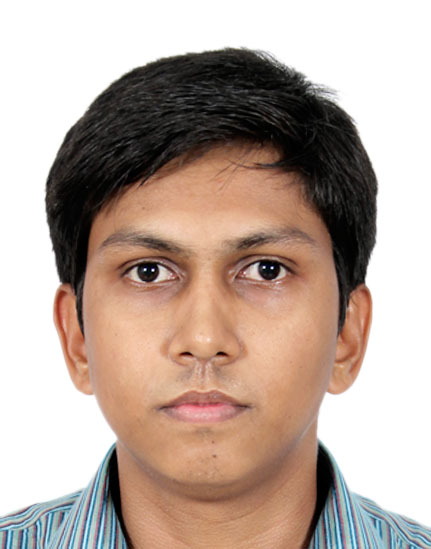
\includegraphics[width=3.6cm, height=3.6cm, keepaspectratio]{profile-picture.jpg}};
                \draw[primary, line width=3pt] (0,0) circle (1.8cm);
            \end{tikzpicture}
        \end{minipage}
    \end{center}
    \vspace{0.3cm}
}

% Skill bar command
\newcommand{\skillbar}[2]{
    \textbf{#1} \\
    \begin{tikzpicture}
        \fill[lightgray] (0,0) rectangle (4,0.2);
        \fill[primary] (0,0) rectangle (#2*4/5,0.2);
    \end{tikzpicture}
    \vspace{2pt}
}

%-------------------------------------------
%%%%%%  RESUME STARTS HERE  %%%%%%%%%%%%%%%%%%%%%%%%%%%%
%-------------------------------------------

\begin{document}

\makeheader

%----------- EXECUTIVE SUMMARY -----------
\section{Executive Summary}
\justifying
\small Engineering educator and R\&D professional with \textbf{9+ years} of comprehensive experience spanning electronics hardware development, embedded systems, AI/ML, and full-stack software engineering. Currently pursuing \textbf{BS in Data Science and Applications from IIT Madras} (Diploma in Programming completed). Distinguished by exceptional student mentorship resulting in \textbf{Rs. 45+ lakhs in innovation funding}, including successful Shark Tank India pitches. Proven expertise in bridging academia-industry gap through innovative teaching methodologies, infrastructure leadership, and real-world system development.

%----------- PROFESSIONAL OBJECTIVES -----------
\section{Professional Objectives}
\small
\begin{itemize}[leftmargin=0.15in, label={}]
    \item \textbf{\color{primary}Immediate Goal:} Secure AICTE Industry Fellowship to gain advanced industrial research experience in AI, embedded computing, or system design, bridging academic excellence with industry innovation
    \item \textbf{\color{primary}Long-term Vision:} Pursue PhD in AI/Embedded Computing/System Design from premier institution while establishing Gujarat as a leading hub for diploma-level innovation and research-driven education
    \item \textbf{\color{primary}Impact Mission:} Transform technical education landscape by integrating industrial rigor with academic excellence, fostering sustainable innovation ecosystems, and creating scalable models for interdisciplinary collaboration
\end{itemize}

%----------- PROFESSIONAL EXPERIENCE -----------
\section{Professional Experience}
\resumeSubHeadingListStart

\resumeSubheading
{Lecturer (Class - II) \& Innovation Leader}{Nov 2016 -- Present}
{Government Polytechnic, Education Department - Government of Gujarat}{Palanpur, Gujarat}
\resumeItemListStart
\resumeItem{Lead comprehensive technical education across Programming in C, Microprocessor Programming, Embedded Systems, Circuit Design, Consumer Electronics, and Entrepreneurship}
\resumeItem{Hold key institutional positions: \textbf{IT Convener} (infrastructure strategy), \textbf{SSIP Co-Convener} (startup ecosystem), \textbf{Training \& Placement Member}, and active contributor to MIS and UDAYAM initiatives}
\resumeItem{Achieved remarkable student success: mentored teams securing \textbf{Rs. 25+ lakhs from Shark Tank India} and \textbf{Rs. 20 lakhs through government innovation programs}, resulting in \textbf{2 student patents}}
\resumeItem{Architected and deployed \textbf{Next.js-based Smart Academic Portal} featuring AI-driven attendance tracking, automated assessment workflows, comprehensive committee management, and real-time analytics dashboard}
\resumeItem{Designed enterprise-grade infrastructure: self-hosted Linux servers, Dockerized microservices, CI/CD pipelines, and automated backup systems}
\resumeItem{Transformed institutional technology landscape while fostering innovation culture and industry partnerships}
\resumeItemListEnd

\resumeSubheading
{Electronics \& Communication Engineer (R\&D)}{Jul 2015 -- Oct 2016}
{TEXEG India Private Limited (Japan-based Technology Firm)}{Gandhinagar, Gujarat}
\resumeItemListStart
\resumeItem{Led end-to-end product development lifecycle for commercial embedded systems in international R\&D environment}
\resumeItem{Executed circuit simulation, PCB design, firmware development, and control systems implementation}
\resumeItem{Designed control algorithms (PID, PI, Fuzzy Logic) using MATLAB Control System Toolbox for industrial applications}
\resumeItem{Delivered complete embedded solutions from concept to production, supporting cross-functional mechanical engineering teams}
\resumeItem{Contributed to innovative product portfolio serving global markets with cutting-edge automation solutions}
\resumeItemListEnd

\resumeSubheading
{Research \& Development Intern}{Aug 2014 -- Jul 2015}
{eiTRA - eInfochips Training \& Research Academy Ltd}{Ahmedabad, Gujarat}
\resumeItemListStart
\resumeItem{Gained comprehensive foundation in embedded systems research methodologies and industry best practices}
\resumeItem{Developed proficiency in advanced debugging techniques and hardware-software integration strategies}
\resumeItemListEnd

\resumeSubHeadingListEnd

%----------- TECHNICAL EXPERTISE -----------
\section{Technical Expertise}
\begin{multicols}{2}
\small

\textbf{Programming Languages:}
\begin{itemize}[leftmargin=15pt, noitemsep, topsep=1pt]
    \item Java, Python, JavaScript (ES6+), C/C++
    \item R, SQL, Assembly Language
    \item HTML5, CSS3, Markdown
\end{itemize}

\textbf{Web \& Full-Stack Development:}
\begin{itemize}[leftmargin=15pt, noitemsep, topsep=1pt]
    \item Next.js, React.js, Vue.js 3
    \item Node.js, Express.js, Flask, FastAPI
    \item RESTful APIs, JWT Authentication
    \item SQLite, MongoDB, PostgreSQL
    \item Redis, Celery, ElasticSearch 
\end{itemize}

\textbf{Data Science \& Machine Learning:}
\begin{itemize}[leftmargin=15pt, noitemsep, topsep=1pt]
    \item TensorFlow, PyTorch, Scikit-learn
    \item Pandas, NumPy, Matplotlib, Seaborn
    \item Computer Vision, NLP, Deep Learning
    \item Recommender Systems, Clustering
\end{itemize}

\textbf{Infrastructure \& DevOps:}
\begin{itemize}[leftmargin=15pt, noitemsep, topsep=1pt]
    \item Linux Server Administration (Ubuntu, CentOS)
    \item Docker, CI/CD Pipelines
    \item Git Version Control, GitHub Actions
    \item Self-hosted \& Cloud Solutions
\end{itemize}

\textbf{Embedded Systems \& Hardware:}
\begin{itemize}[leftmargin=15pt, noitemsep, topsep=1pt]
    \item 8051, PIC, AVR Microcontrollers
    \item STM32, Arduino, Raspberry Pi, ESP8266
    \item EagleCAD, Altium, OrCAD, KiCAD
    \item Multisim, Proteus, LTspice
\end{itemize}

\textbf{Engineering Tools \& Platforms:}
\begin{itemize}[leftmargin=15pt, noitemsep, topsep=1pt]
    \item MATLAB, Simulink, Control Systems
    \item FPGA Design, Verilog, Digital Design
    \item Signal \& Image Processing
    \item CAD Tools, Circuit Simulation
    \item Modbus Protocol, Industrial Automation
\end{itemize}

\end{multicols}

%----------- EDUCATION -----------
\section{Education}
\resumeSubHeadingListStart

\resumeSubheading
{Bachelor of Science (BS) in Data Science and Applications}{2021 -- Present}
{Indian Institute of Technology Madras (IIT Madras)}{Online Program}
\resumeItemListStart
\resumeItem{\textbf{Diploma in Programming} - Successfully Completed with Distinction}
\resumeItem{\textbf{Diploma in Data Science} - Final project phase (95\% completion)}
\resumeItem{Comprehensive coursework: Advanced Statistics, Machine Learning, Deep Learning, Data Visualization, Big Data Analytics}
\resumeItemListEnd

\resumeSubheading
{Master of Engineering(ME), Communication Systems}{2013 -- 2015}
{L.D College of Engineering, Gujarat Technological University}{Ahmedabad, Gujarat}
\resumeItemListStart
\resumeItem{Specialized in Digital Signal Processing, Wireless Communications, and Advanced Communication Protocols}
\resumeItemListEnd

\resumeSubheading
{Bachelor of Engineering(BE), Electronics \& Communication}{2009 -- 2013}
{Sal Institute of Technology and Engineering Research, Gujarat Technological University}{Gujarat}
\resumeItemListStart
\resumeItem{Foundation in Electronics Design, Embedded Systems, and Communication Technologies}
\resumeItemListEnd

\resumeSubHeadingListEnd

%----------- PROFESSIONAL CERTIFICATIONS -----------
\section{Professional Certifications}
\resumeSubHeadingListStart

\resumeProjectHeading
{\textbf{\href{https://www.coursera.org/user/e52746bb9f0640066b270cdc17eb7c6a}{Coursera Specializations}}}{2016 -- Present}
\resumeItemListStart
\resumeItem{\textbf{\href{https://www.coursera.org/account/accomplishments/specialization/certificate/JKAWDXLZWMEB}{Advanced Machine Learning}:} \href{https://www.coursera.org/account/accomplishments/certificate/SPLQ5CYQVWKN}{Introduction to Deep Learning} | \href{https://www.coursera.org/account/accomplishments/certificate/7LFSTE9FPBXM}{Data Science Competition} | \href{https://www.coursera.org/account/accomplishments/certificate/985PD2B7VE23}{Bayesian Methods} | \href{https://www.coursera.org/account/accomplishments/certificate/CK3QW97WNZKB}{Reinforcement Learning} | \href{https://www.coursera.org/account/accomplishments/certificate/W5DWR22MF3A5}{Computer Vision} | \href{https://www.coursera.org/account/accomplishments/certificate/HVV4QA3FSDTM}{NLP} | \href{https://www.coursera.org/account/accomplishments/certificate/XXM674GHFURX}{LHC Machine Learning}}

\resumeItem{\textbf{\href{https://www.coursera.org/account/accomplishments/specialization/certificate/THHR93FYA8SH}{Machine Learning}:} \href{https://www.coursera.org/account/accomplishments/certificate/Q5FYFEYGC5UG}{ML Foundations} | \href{https://www.coursera.org/account/accomplishments/certificate/QUS878PRPRC9}{ML Regression} | \href{https://www.coursera.org/account/accomplishments/certificate/HDJMXPU25AVZ}{ML Classification} | \href{https://www.coursera.org/account/accomplishments/certificate/AXYBJPXP3QE6}{ML Clustering \& Retrieval}}

\resumeItem{\textbf{\href{https://www.coursera.org/account/accomplishments/specialization/certificate/Z9V42UF7JDFE}{Deep Learning}:} \href{https://www.coursera.org/account/accomplishments/certificate/8BQPBRCZULZU}{Neural Networks \& Deep Learning} | \href{https://www.coursera.org/account/accomplishments/certificate/7TD3GGF2PM94}{Hyperparameter Tuning} | \href{https://www.coursera.org/account/accomplishments/certificate/9M54F4EB6LS9}{ML Projects} | \href{https://www.coursera.org/account/accomplishments/certificate/3ZUKLU6PWBY2}{CNNs} | \href{https://www.coursera.org/account/accomplishments/certificate/4U46X46HL6B3}{Sequence Models}}

\resumeItem{\textbf{\href{https://www.coursera.org/account/accomplishments/specialization/certificate/SZPEUACNCHKY}{Recommender Systems}:} \href{https://www.coursera.org/account/accomplishments/certificate/WQA5MFK3VFBB}{Non-Personalized Systems} | \href{https://www.coursera.org/account/accomplishments/certificate/4SZA4D696B6C}{Collaborative Filtering} | \href{https://www.coursera.org/account/accomplishments/certificate/BHNC2YX9BQSX}{Evaluation \& Metrics} | \href{https://www.coursera.org/account/accomplishments/certificate/JQM7FHL99WCA}{Matrix Factorization} | \href{https://www.coursera.org/account/accomplishments/certificate/CZV2FDRHAHDV}{Capstone Project}}

\resumeItem{\textbf{Data Structures and Algorithms:} \href{https://www.coursera.org/account/accomplishments/certificate/2TBS3B7SR6BW}{Algorithmic Toolbox} | \href{https://www.coursera.org/account/accomplishments/certificate/626PE4897FKU}{Data Structures} | \href{https://www.coursera.org/account/accomplishments/certificate/SMEPD4F5RUZT}{Algorithms on Graphs} | \href{https://www.coursera.org/account/accomplishments/certificate/C3WFWJQQ3B8U}{Algorithms on Strings} | \href{https://www.coursera.org/account/accomplishments/certificate/4PAYHQXURE95}{Genome Assembly}}

\resumeItem{\textbf{Big Data:} \href{https://www.coursera.org/account/accomplishments/certificate/BP6LAGC7RM5Z}{Introduction to Big Data} | \href{https://www.coursera.org/account/accomplishments/certificate/3RZZQU95SQY7}{Big Data Modeling} | \href{https://www.coursera.org/account/accomplishments/certificate/QUQCX6WNBK5U}{Big Data Integration} | \href{https://www.coursera.org/account/accomplishments/records/QW6W7R9DUWJ2}{ML with Big Data} | \href{https://www.coursera.org/account/accomplishments/certificate/2S46AN2CM9P9}{Graph Analytics}}

\resumeItem{\textbf{Data Mining:} \href{https://www.coursera.org/account/accomplishments/certificate/7HF8N8Q6ENDH}{Data Visualization} | \href{https://www.coursera.org/account/accomplishments/certificate/44FTGM4VGWJW}{Text Retrieval} | \href{https://www.coursera.org/account/accomplishments/certificate/XXSKFSC9FXZP}{Text Mining} | \href{https://www.coursera.org/account/accomplishments/certificate/SFBWR7HF4RXC}{Pattern Discovery} | \href{https://www.coursera.org/account/accomplishments/certificate/9ZAVTE8KM5UP}{Cluster Analysis}}

\resumeItem{\textbf{Cloud Computing:} \href{https://www.coursera.org/account/accomplishments/certificate/VN2ME8K8DZ87}{Cloud Systems \& Infrastructure} | \href{https://www.coursera.org/account/accomplishments/records/Y956NGS7N3VF}{Big Data Applications in Cloud}}

\resumeItem{\textbf{Android Development:} \href{https://www.coursera.org/account/accomplishments/certificate/P3BAZCKJGW66}{Java for Android}}
\resumeItemListEnd

\resumeProjectHeading
{\textbf{NPTEL Excellence \& Recognition}}{2018 -- Present}
\resumeItemListStart
\resumeItem{\textbf{Foundations of Computing:} Discrete Mathematics (2021) | Design and Analysis of Algorithms (2020) - Elite | Programming, Data Structures and Algorithms Using Python (2020) - Elite | Computer Graphics (2020)}

\resumeItem{\textbf{Systems Domain:} Operating System (2020) - Elite | Computer Networks and Internet Protocol (2018) | Database Management System (2020) - Elite | Introduction to Internet of Things (2018) - Elite | Cloud Computing (2020) - Elite | Computer Architecture and Organization (2020)}

\resumeItem{\textbf{Programming Languages:} Programming in Java (2020) - Elite + Gold | Joy of Computing Using Python (2019) - Elite + Silver | Introduction to R Software (2019) - Elite + Silver}

\resumeItem{\textbf{Machine Learning \& AI:} Introduction to Machine Learning (2019) - Elite + Silver | Deep Learning - Part 1 (2019) - Elite + Silver | Reinforcement Learning (2019) - Elite}

\resumeItem{\textbf{Data Science \& Analytics:} Data Science for Engineers (2019) - Elite + Silver | Business Analytics and Data Mining Modeling Using R (2019) - Elite + Silver | Business Analytics \& Data Mining Modeling Using R - Part II (2018) - Elite | Business Analytics \& Text Mining Modeling Using Python (2019) - Elite + Silver | Business Statistics (2019) - Elite | Scalable Data Science (2018)}

\resumeItem{\textbf{Industry 4.0 \& IoT:} Introduction to Industry 4.0 and Industrial IoT (2019) - Elite}

\resumeItemListEnd

\resumeProjectHeading
{\textbf{Udemy Professional Development}}{2017 -- Present}
\resumeItemListStart
\resumeItem{\textbf{\href{https://www.udemy.com/certificate/UC-RL1GE2YN/}{CCNA Routing and Switching}} - Network Infrastructure, Routing Protocols, Switching}
\resumeItem{\textbf{\href{https://www.udemy.com/certificate/UC-2TYO3NTA/}{Machine Learning and Data Science}} - Python \& R for Data Science, ML Applications}
\resumeItem{\textbf{\href{http://ude.my/UC-K94NR7NJ}{Complete Python Masterclass}} - Python Programming, Applications, Best Practices}
\resumeItem{\textbf{\href{https://www.udemy.com/certificate/UC-IQTMC465/}{Complete JavaScript Course}} - Web Development, JavaScript Programming}
\resumeItem{\textbf{\href{http://ude.my/UC-JS1BBZG3}{MBA in 1 Course}} - Business Fundamentals, Management Principles}
\resumeItemListEnd

\resumeSubHeadingListEnd

%----------- KEY PROJECTS & INNOVATIONS -----------
\section{Key Projects \& Innovations}
\resumeSubHeadingListStart

\resumeProjectHeading
{\textbf{Smart Academic Portal} \textit{| Next.js, React, Docker}}{2023 -- Present}
\resumeItemListStart
\resumeItem{Architected comprehensive academic management ecosystem serving 500+ students and 50+ faculty members}
\resumeItem{Implemented AI-powered attendance tracking with 98\% accuracy, reducing administrative overhead by 60\%}
\resumeItem{Built automated assessment pipeline with real-time analytics, improving result processing efficiency by 75\%}
\resumeItem{Deployed on self-managed cloud infrastructure with 99.9\% uptime, zero-downtime deployments, and automated scaling}
\resumeItem{Enabled collaborative development model with student contributors, fostering practical learning experiences}
\resumeItemListEnd


\resumeProjectHeading
{\textbf{Scarlett Web Application (MAD1)} \textit{| Flask, SQLAlchemy}}{2022 -- 2023}
\resumeItemListStart
\resumeItem{Developed comprehensive web application for household service booking and management with multi-role system}
\resumeItem{Implemented three distinct user roles (Customer, Professional, Admin) with specialized interfaces and permissions}
\resumeItem{Built professional verification system with customer review, rating functionality, and document upload capabilities}
\resumeItem{Integrated Flask-Security for robust authentication, authorization, and role-based access control}
\resumeItem{Created comprehensive admin panel for user verification, service management, and system statistics}
\resumeItemListEnd

\resumeProjectHeading
{\textbf{Scarlett Web Application (MAD2)} \textit{| Vue.js, Flask, PostgreSQL}}{2023 -- 2024}
\resumeItemListStart
\resumeItem{Enhanced household services platform with modern Vue.js 3 frontend architecture and advanced backend processing}
\resumeItem{Implemented microservices-style API structure with dedicated modules for comprehensive functionality}
\resumeItem{Integrated Celery with Redis for asynchronous task handling and background processing capabilities}
\resumeItem{Built comprehensive analytics and reporting system with Chart.js visualizations and real-time data}
\resumeItem{Developed RESTful API following industry best practices with JWT-based authentication system}
\resumeItemListEnd

\resumeProjectHeading
{\textbf{FPGA Image Steganography} \textit{| FPGA, Verilog, DSP}}{2015}
\resumeItemListStart
\resumeItem{Developed hardware implementation of YASS (Yet Another Steganographic Scheme) for secure communication}
\resumeItem{Implemented resistance to self-calibration based blind steganalysis attacks using advanced algorithms}
\resumeItem{Utilized FPGA technology for real-time image processing and steganographic embedding}
\resumeItem{Published in International Journal of Computer Applications - \href{https://www.ijcaonline.org/archives/volume120/number9/21259-4125}{\textcolor{primary}{View Research Paper}}}
\resumeItemListEnd

\resumeProjectHeading
{\textbf{Wireless Data Acquisition System} \textit{| Modbus, Embedded Systems}}{2015 -- 2016}
\resumeItemListStart
\resumeItem{Designed multi-device wireless monitoring and control system for industrial applications}
\resumeItem{Implemented Modbus protocol for reliable communication with up to 255 devices}
\resumeItem{Developed real-time data processing capabilities for industrial monitoring and environmental sensing}
\resumeItem{Applied in process control, environmental monitoring, and industrial automation systems}
\resumeItemListEnd

\resumeSubHeadingListEnd

%----------- ACHIEVEMENTS & RECOGNITION -----------
\section{Achievements \& Recognition}
\resumeSubHeadingListStart

\resumeProjectHeading
{\textbf{Student Innovation Mentorship Excellence}}{2018 -- Present}
\resumeItemListStart
\resumeItem{Established comprehensive innovation pipeline from ideation to commercialization, mentoring 50+ student projects}
\resumeItem{Guided breakthrough projects: IoT-based smart agriculture system, autonomous drone delivery platform, embedded automation solutions}
\resumeItem{Achieved exceptional funding success: \textbf{Rs. 25 lakhs from Shark Tank India} and \textbf{Rs. 20 lakhs government grants}}
\resumeItem{Resulted in \textbf{2 filed patents} and multiple technology transfer opportunities with industry partners}
\resumeItem{Created sustainable mentorship model adopted across multiple institutions in Gujarat}
\resumeItemListEnd

\resumeProjectHeading
{\textbf{NPTEL Excellence \& Recognition}}{2018 -- Present}
\resumeItemListStart
\resumeItem{\textbf{NPTEL EVANGELIST} (Dec 2020) - Top recognition for exceptional contribution to online learning ecosystem}
\resumeItem{\textbf{NPTEL DISCIPLINE STAR - Computer Science} (Dec 2019, Dec 2020) - Top 1\% performer nationally}
\resumeItem{\textbf{NPTEL ENTHUSIAST \& MOTIVATED LEARNER} (Dec 2019, Dec 2020) - Consistent excellence in learning}
\resumeItem{\textbf{NPTEL BELIEVER} (Jul-Dec 2019, Jan-Apr 2020, Jul-Dec 2020) - Sustained engagement and performance}
\resumeItem{\textbf{24 Course Completions with 15 Elite Performances} - Demonstrating mastery across diverse technical domains}
\resumeItemListEnd

\resumeSubHeadingListEnd

\end{document}
